\section{Method}
\label{sec:method}
\label{sec:backbone}

\method{} learns tissue descriptions and their cross-granularity transformations from nested observations (Figure~\ref{fig:method}). Molecular--spatial learning retains information within each neighborhood, while a shared continuous transformation predicts how its molecular description changes with the amount of surrounding context.

\begin{figure}[t]
\centering
\resizebox{\linewidth}{!}{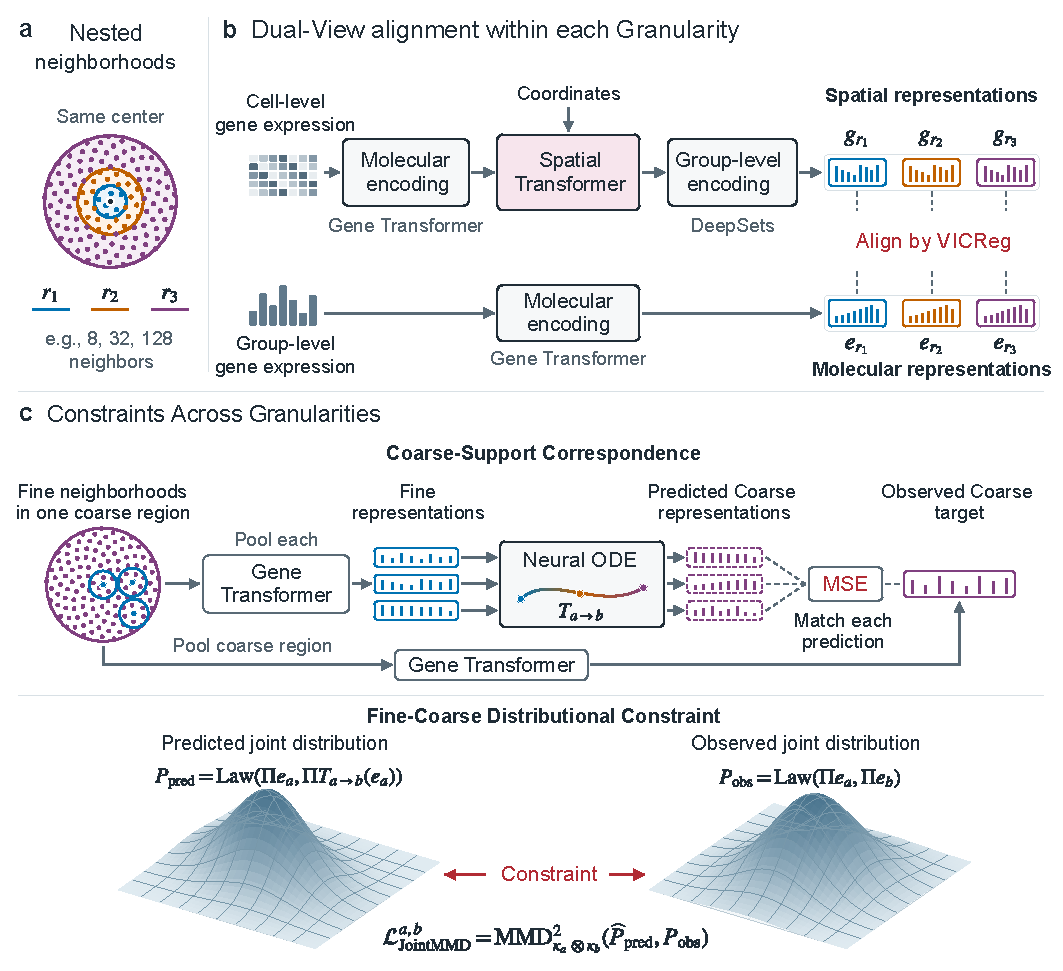
\includegraphics[width=\linewidth]{figures/zoomst_figure1_v5.pdf}
}
\caption{\textbf{ZoomST overview.}
\textbf{a}, Nested neighborhoods share a center and span increasing granularities, here 8, 32 and 128 measured positions.
\textbf{b}, Molecular and spatial encoders produce representations $e_r$ and $g_r$, aligned by VICReg within each granularity and retained for analysis.
\textbf{c}, A shared neural ODE predicts coarser molecular states. Coarse-support MSE compares predictions from fine observations with a common, directly encoded coarse target. Joint MMD compares fine--predicted-coarse pairs with fine--observed-coarse pairs at matched centers.}
\label{fig:method}
\end{figure}

\subsection{Observation granularity and nested tissue context}
\label{sec:nested-observations}

A tissue section contains expression profiles $x_i$ and coordinates $p_i$ at $N$ measured positions, each representing a cell or spatial bin. Let $S_{i,r}$ contain $i$ and its $r-1$ nearest spatial neighbors. The \emph{observation granularity} $r$ counts the positions summarized around $i$; increasing it expands context on the same measurement grid. Training uses nested supports at $r\in\Rset=\{8,32,128\}$. Their molecular profiles average preprocessed expression, $m_{i,r}=r^{-1}\sum_{j\in S_{i,r}}\bar x_j$. Expanding a support retains shared measurements and adds new context, providing paired observations without anatomical labels.

\subsection{Molecular--spatial representations within each granularity}
\label{sec:within-granularity}

The molecular view is $e_{i,r}=E_{\mathrm{PB}}(\operatorname{Tokenize}(m_{i,r}))\in\mathbb R^d$: a pseudobulk Transformer encodes gene identities and discretized expression values after pooling. The spatial view additionally describes arrangement. A position-wise Transformer supplies states $h_j$; a shared spatial Transformer contextualizes them using relative coordinates and a granularity identifier. A shared DeepSets readout~\citep{zaheer2017deepsets} pools the resulting states into $g_{i,r}\in\mathbb R^d$. Both views have $d=256$. The two molecular Transformers have separate parameters and share gene and expression-bin embeddings.

Masked expression reconstruction grounds both views in molecular content: $e_{i,r}$ and $g_{i,r}$ reconstruct the pooled neighborhood profile, alongside reconstruction of the focal observation. The combined reconstruction loss $\mathcal L_{\mathrm{rec}}$ and within-granularity VICReg alignment~\citep{bardes2022vicreg} define $\mathcal L_{\mathrm{base}}$. VICReg's variance and covariance terms regularize the aligned states. Both views remain available; transformations act on $e$, whose observation is the pooled molecular profile. Appendices~\ref{app:preprocessing} and~\ref{app:hyperparameters} specify tokenization, architecture and the base objective.
